\documentclass[11pt]{article}

% Change "review" to "final" to generate the final (sometimes called camera-ready) version.
% Change to "preprint" to generate a non-anonymous version with page numbers.
\usepackage[review]{acl}
\usepackage{amsmath}       % 公式（你已经在用）
\usepackage{amssymb}       % 数学符号
\usepackage{algorithm}     % algorithm环境
\usepackage{algorithmic}   % \STATE 这些
% Standard package includes
\usepackage{times}
\usepackage{latexsym}
\usepackage{tikz}
\usetikzlibrary{positioning,arrows.meta}
% For proper rendering and hyphenation of words containing Latin characters (including in bib files)
\usepackage[T1]{fontenc}
% For Vietnamese characters
% \usepackage[T5]{fontenc}
% See https://www.latex-project.org/help/documentation/encguide.pdf for other character sets

% This assumes your files are encoded as UTF8
\usepackage[utf8]{inputenc}

% This is not strictly necessary, and may be commented out,
% but it will improve the layout of the manuscript,
% and will typically save some space.
\usepackage{microtype}

% This is also not strictly necessary, and may be commented out.
% However, it will improve the aesthetics of text in
% the typewriter font.
\usepackage{inconsolata}

%Including images in your LaTeX document requires adding
%additional package(s)
\usepackage{graphicx}

% If the title and author information does not fit in the area allocated, uncomment the following
%
%\setlength\titlebox{<dim>}
%
% and set <dim> to something 5cm or larger.

\title{Instructions for *ACL Proceedings}

% Author information can be set in various styles:
% For several authors from the same institution:
% \author{Author 1 \and ... \and Author n \\
%         Address line \\ ... \\ Address line}
% if the names do not fit well on one line use
%         Author 1 \\ {\bf Author 2} \\ ... \\ {\bf Author n} \\
% For authors from different institutions:
% \author{Author 1 \\ Address line \\  ... \\ Address line
%         \And  ... \And
%         Author n \\ Address line \\ ... \\ Address line}
% To start a separate ``row'' of authors use \AND, as in
% \author{Author 1 \\ Address line \\  ... \\ Address line
%         \AND
%         Author 2 \\ Address line \\ ... \\ Address line \And
%         Author 3 \\ Address line \\ ... \\ Address line}

\author{First Author \\
  Affiliation / Address line 1 \\
  Affiliation / Address line 2 \\
  Affiliation / Address line 3 \\
  \texttt{email@domain} \\\And
  Second Author \\
  Affiliation / Address line 1 \\
  Affiliation / Address line 2 \\
  Affiliation / Address line 3 \\
  \texttt{email@domain} \\}

%\author{
%  \textbf{First Author\textsuperscript{1}},
%  \textbf{Second Author\textsuperscript{1,2}},
%  \textbf{Third T. Author\textsuperscript{1}},
%  \textbf{Fourth Author\textsuperscript{1}},
%\\
%  \textbf{Fifth Author\textsuperscript{1,2}},
%  \textbf{Sixth Author\textsuperscript{1}},
%  \textbf{Seventh Author\textsuperscript{1}},
%  \textbf{Eighth Author \textsuperscript{1,2,3,4}},
%\\
%  \textbf{Ninth Author\textsuperscript{1}},
%  \textbf{Tenth Author\textsuperscript{1}},
%  \textbf{Eleventh E. Author\textsuperscript{1,2,3,4,5}},
%  \textbf{Twelfth Author\textsuperscript{1}},
%\\
%  \textbf{Thirteenth Author\textsuperscript{3}},
%  \textbf{Fourteenth F. Author\textsuperscript{2,4}},
%  \textbf{Fifteenth Author\textsuperscript{1}},
%  \textbf{Sixteenth Author\textsuperscript{1}},
%\\
%  \textbf{Seventeenth S. Author\textsuperscript{4,5}},
%  \textbf{Eighteenth Author\textsuperscript{3,4}},
%  \textbf{Nineteenth N. Author\textsuperscript{2,5}},
%  \textbf{Twentieth Author\textsuperscript{1}}
%\\
%\\
%  \textsuperscript{1}Affiliation 1,
%  \textsuperscript{2}Affiliation 2,
%  \textsuperscript{3}Affiliation 3,
%  \textsuperscript{4}Affiliation 4,
%  \textsuperscript{5}Affiliation 5
%\\
%  \small{
%    \textbf{Correspondence:} \href{mailto:email@domain}{email@domain}
%  }
%}

\begin{document}
\maketitle
\begin{abstract}
This document is a supplement to the general instructions for *ACL authors. It contains instructions for using the \LaTeX{} style files for ACL conferences.
The document itself conforms to its own specifications, and is therefore an example of what your manuscript should look like.
These instructions should be used both for papers submitted for review and for final versions of accepted papers.
\end{abstract}

\section{Introduction}
\label{sec:intro}

Human affect is expressed through multiple channels: lexical choice, prosody,
facial motion, and context~\citep{zadeh2017tensor,zadeh2018multi}.
Multimodal sentiment analysis (MSA) therefore seeks functions that map
heterogeneous sequences to scalar or ordinal sentiment labels while respecting
asynchrony and uneven sensor reliability~\citep{tsai2019multimodal}.

Deep fusion models can exploit statistical cues that are predictive on the
training distribution yet brittle under shift: when acoustic or visual streams
are noisy, standard cross-modal attention still assigns non-negligible mass to
spurious key positions, propagating variance into the joint representation.
Information bottleneck (IB) objectives offer a principled remedy by encouraging
representations that retain predictive information while discarding nuisance
factors~\citep{alemi2017deep}.
Prior MSA systems explored modality-invariant and modality-specific
subspaces~\citep{hazarika2020misa,yu2021learning}, hierarchical mutual-information
objectives~\citep{han2021improving}, and causal or debiased variants such as
CaMIB~\citep{jiang2025towards}.
Yet these methods typically fuse modalities before or in parallel with
compression, commit predictions to a statically chosen textual ``highway'', and
do not make fusion aware of per-token uncertainty~\citep{yang2025improving}.

To address these challenges, we propose PRISM, a primary-centric
MSA framework that fuses modalities only after IB-style compression and makes
fusion explicitly aware of per-token uncertainty.
Specifically, each modality is first encoded into a bottleneck through
variational IB encoders with Gaussian reparameterization, so that a
per-token confidence signal derived from IB uncertainty
becomes available to downstream attention.
Next, a differentiable MSelector assigns a per-sample primary modality
via Gumbel--Softmax routing, so that only the fused \emph{primary} bottleneck
is pooled and passed to the regression head---no direct textual shortcut into
the classifier, aligning with primary-centric designs in recent
modality-optimization work~\citep{yang2025improving}.
Finally, InfoGate layers apply confidence-biased cross-modal attention
and adaptive gates to rescale auxiliary contributions using primary context.
A two-stage curriculum separates IB warm-up from routing supervision, in which
stage-two KL targets align routing weights with per-modality predictive errors.

We conduct extensive experiments on three standard MSA benchmarks (CMU-MOSI,
CMU-MOSEI, and CH-SIMS v2), together with a large-scale Optuna hyperparameter
study. Empirical results and analyses validate the effectiveness of PRISM
under complete-modality protocols.

\section{Related Work}
\label{sec:related}

\noindent \textbf{Transformer-based fusion}.
MulT \citep{tsai2019multimodal} stacks cross-modal attention blocks for unaligned
MSA; MAG-BERT \citep{rahman2020integrating} injects nonverbal context into
language models.
These models typically form a \emph{single} fused representation before the head.
PRISM instead keeps an explicit primary vs.\ auxiliary asymmetry after IB
compression.

\noindent \textbf{Modality-specific representation learning}.
MISA \citep{hazarika2020misa} disentangles invariant and specific factors; Self-MM
\citep{yu2021learning} adds self-supervision.
PRISM is complementary: we do not maintain parallel invariant/specific
towers, but we \emph{do} enforce per-modality bottlenecks with shared
dimensionality before fusion.

\noindent \textbf{Information bottlenecks and debiasing}.
Deep variational IB \citep{alemi2017deep} motivates stochastic encoders; CaMIB
\citep{jiang2025towards} combines IB-style filtering with causal masks for OOD
robustness.
PRISM is \emph{not} a causal identification paper; rather, we use IB
confidence as a \emph{mechanistic} control signal inside attention, closer to
uncertainty-aware fusion than to full causal graphs.

\noindent \textbf{Dynamic primary modality selection}.
Lines of work on modality optimization and dynamic primaries
\citep{mods2026align,yang2025improving} argue that the ``best'' carrier modality varies by sample.
Our MSelector realizes this with lightweight pooling scores and Gumbel--Softmax
gradients, with stage-two KL targets derived from per-modality label prediction
errors (``select the modality that already fits the label'').

\noindent \textbf{Conceptual connections to hierarchical and token-level IB}.
Hierarchical IB fusion \citep{ithp2024align} and token-level IB perspectives
\citep{cyin2025align} informed exploratory designs; we cite them as internal
alignment references and emphasize that PRISM's implementation is
self-contained and should be evaluated on its own merits.

\section{Methodology}
\label{sec:methodology}

\subsection{Positioning relative to MODS and CyIN}
\label{sec:mods-cyin-positioning}

\textbf{MODS.}
MODS \citep{mods2026align} advocates modality optimization with a
\emph{sample-dependent} primary stream: the model should not assume that text
always carries the decisive evidence, and fusion should be organized around
whichever modality best supports the label for each instance.
PRISM adopts the same high-level stance through MSelector
(\S\ref{sec:method-msel}), but instantiates it on \emph{IB-compressed}
bottlenecks rather than on raw modality streams, and routes the final
prediction exclusively through the enhanced primary bottleneck (no direct
textual shortcut into the head), which matches the primary-centric design
discipline emphasized in recent modality-optimization work
\citep{yang2025improving}.

\textbf{CyIN.}
CyIN \citep{cyin2025align} motivates token-level information bottlenecks and
informative latent spaces that suppress nuisance variation while retaining
task-relevant structure.
PRISM is aligned with that goal in that each modality passes through a
stochastic bottleneck whose variance supplies a per-token confidence map, but
differs in \emph{where} that signal is consumed: we use IB uncertainty to bias
cross-modal attention and gates inside InfoGate (\S\ref{sec:method-layer}),
rather than treating the bottleneck solely as a standalone encoder objective.

\textbf{Synthesis.}
Together, MODS-style primary routing and CyIN-style token-level compression
inform PRISM's training story---IB warm-up, differentiable primary selection,
routing supervision, and confidence-aware fusion---but the implementation and
evaluation protocol below are self-contained.

\subsection{Problem Formulation}
\label{sec:method-problem}

We study multimodal sentiment analysis (MSA) as the main task of this work.
Given an utterance-level video segment, the model receives three aligned
modalities: language ($t$), acoustic ($a$), and visual ($v$). The goal is to
predict a continuous sentiment score $y \in \mathbb{R}$.

Let $(X_t, X_a, X_v)$ denote the input modalities. We formulate MSA as a
regression problem and learn a predictor
\begin{equation}
\hat{y} = f_{\theta}(X_t, X_a, X_v),
\end{equation}
where $\hat{y}$ is the predicted sentiment score and $\theta$ denotes all
trainable parameters.

A key challenge in multimodal regression is that modality reliability varies
across samples. In some cases, language provides explicit sentiment evidence;
in others, acoustic tone or facial expressions may be more informative.
Moreover, noisy or redundant modality-specific features can mislead
cross-modal fusion. Therefore, a desirable multimodal regressor should not
only integrate multiple modalities, but also identify which modality should
serve as the main evidence source for each sample.

To this end, we propose \textbf{PRISM}, a primary-modality-centered framework.
For MSA, PRISM first compresses each modality into an information bottleneck
representation, dynamically selects a primary modality, performs
confidence-aware fusion around the selected primary stream, and finally
predicts the regression score from the enhanced primary representation.
We first present PRISM under the MSA regression setting, and then describe its
extension to classification-based affective tasks in
\S\ref{sec:method-cls}.

\subsection{Overview of PRISM}
\label{sec:method-overview}

The overall architecture of PRISM is shown in Figure~\ref{fig:arch} and
summarized in Algorithm~\ref{alg:forward}. For MSA, the modality set is
$\mathcal{M}_{\mathrm{reg}}=\{t,a,v\}$.

First, each modality is projected into a unified representation space and
encoded by a modality-specific information bottleneck (IB) encoder. For the
language modality, PRISM uses a pretrained language model as the text encoder;
for acoustic and visual modalities, lightweight projectors are used to map
features into the shared hidden space. The IB encoder produces a bottleneck
sequence $\mathbf{B}_m$ and a confidence map $\mathbf{C}_m$ for each modality
$m$. The confidence map is derived from the estimated bottleneck variance and
is used to measure token-level reliability.

Second, PRISM uses a dynamic primary modality selector, denoted as
\textbf{MSelector}, to determine the primary modality for each sample. The
selected primary stream is treated as the central prediction path, while the
remaining modalities are routed as auxiliary sources.

Third, stacked InfoGate layers perform asymmetric multimodal fusion. Instead
of concatenating or symmetrically attending over all modalities, InfoGate uses
auxiliary modalities to refine the primary stream. During this process,
confidence maps suppress uncertain tokens and reduce the impact of noisy
features.

Finally, the enhanced primary representation
$\mathbf{B}_p^{\mathrm{out}}$ is pooled and fed into a task head to obtain the
final prediction. In the regression setting, this head outputs a continuous
sentiment score.

\begin{figure}[t]
  \centering
  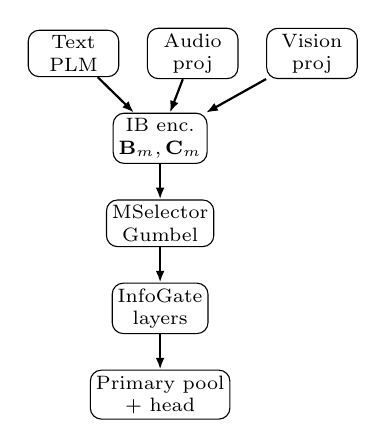
\begin{tikzpicture}[
    font=\scriptsize,
    box/.style={draw, rounded corners, align=center, inner sep=2pt, minimum width=1.15cm},
    arr/.style={-{Latex[length=1.5mm]}, thick}
  ]
    \node[box] (t) {Text\\PLM};
    \node[box, right=0.35cm of t] (a) {Audio\\proj};
    \node[box, right=0.35cm of a] (v) {Vision\\proj};
    \node[box, below=0.45cm of t, xshift=1.1cm] (ib) {IB enc.\\$\mathbf{B}_m,\mathbf{C}_m$};
    \node[box, below=0.45cm of ib] (ms) {MSelector\\Gumbel};
    \node[box, below=0.45cm of ms] (ig) {InfoGate\\layers};
    \node[box, below=0.45cm of ig] (hd) {Primary pool\\+ head};
    \draw[arr] (t) -- (ib);
    \draw[arr] (a) -- (ib);
    \draw[arr] (v) -- (ib);
    \draw[arr] (ib) -- (ms);
    \draw[arr] (ms) -- (ig);
    \draw[arr] (ig) -- (hd);
  \end{tikzpicture}
  \caption{The overall architecture of PRISM under the MSA regression setting.
  Each modality is encoded into an IB bottleneck with confidence estimation.
  MSelector dynamically selects the primary modality, and stacked InfoGate
  layers perform confidence-aware fusion before primary-only prediction.}
  \label{fig:arch}
\end{figure}

\begin{algorithm}[t]
  \caption{PRISM forward pass on a batch.}
  \label{alg:forward}
  \begin{algorithmic}[1]
    \STATE Encode modality-specific features
    $\mathbf{F}_m \rightarrow (\mathbf{B}_m, \mathbf{C}_m)$
    for $m \in \mathcal{M}$.
    \STATE Compute token-level and label-level IB objectives:
    $\mathcal{L}_{\mathrm{tib}}$ and $\mathcal{L}_{\mathrm{lib}}$.
    \STATE Obtain routing weights and hard selection
    $(w,r) \leftarrow \mathrm{MSelector}(\{\mathbf{B}_m\}_{m\in\mathcal{M}})$.
    \STATE Route primary and auxiliary bottlenecks
    $(\mathbf{B}_p,\mathbf{C}_p,\mathcal{A})
    \leftarrow \mathrm{Route}(\mathbf{B}_m,\mathbf{C}_m,w,r)$.
    \STATE Refine primary representation via InfoGate
    $\mathbf{B}_p^{\mathrm{out}} \leftarrow
    \mathrm{InfoGateStack}(\mathbf{B}_p,\mathbf{C}_p,\mathcal{A})$.
    \STATE Predict output
    $\hat{y} \leftarrow
    \mathrm{Head}(\mathrm{Pool}(\mathbf{B}_p^{\mathrm{out}}))$.
    \STATE $\mathcal{L}_{\mathrm{rib}} \leftarrow 0$.
    \IF{$\mathrm{epoch} > E_{\mathrm{warmup}}$}
      \STATE Update routing supervision $\mathcal{L}_{\mathrm{rib}}$.
    \ENDIF
    \RETURN $\hat{y}$,
    $\mathcal{L}_{\mathrm{tib}}+\mathcal{L}_{\mathrm{lib}}$,
    $\mathcal{L}_{\mathrm{rib}}$.
  \end{algorithmic}
\end{algorithm}

Here, $\mathcal{A}$ denotes the set of routed auxiliary modality bottlenecks
and confidence maps. In the three-modality regression setting,
$\mathcal{A}=\{(\mathbf{B}_{a_1},\mathbf{C}_{a_1}),
(\mathbf{B}_{a_2},\mathbf{C}_{a_2})\}$.

\subsection{Information-Bottleneck Representation Learning}
\label{sec:method-ibenc}

We first project the language, acoustic, and visual inputs into a shared
feature space. Let
$\mathbf{F}_m \in \mathbb{R}^{N \times T \times d}$ denote the projected
feature sequence of modality $m$, where $N$ is the batch size, $T$ is the
sequence length, and $d$ is the unified hidden dimension.

Directly fusing these features may introduce modality-specific noise into the
prediction process. To improve robustness, we encode each modality with a
variational IB encoder. The encoder compresses the original feature sequence
into a bottleneck representation while estimating its uncertainty. For each
modality, the IB encoder predicts a Gaussian mean and log-variance:
\begin{equation}
[\boldsymbol{\mu}_m;\log\boldsymbol{\sigma}_m^2]
=
\mathrm{IBEnc}_m(\mathbf{F}_m).
\end{equation}

During training, the bottleneck representation is sampled using the
reparameterization trick:
\begin{equation}
\begin{aligned}
\mathbf{B}_m
&=
\boldsymbol{\mu}_m
+
\boldsymbol{\epsilon}
\odot
\exp\!\left(\tfrac{1}{2}\log\boldsymbol{\sigma}_m^2\right), \\
\boldsymbol{\epsilon}
&\sim \mathcal{N}(\mathbf{0},\mathbf{I}).
\end{aligned}
\end{equation}
At inference time, we use the deterministic mean representation
$\mathbf{B}_m=\boldsymbol{\mu}_m$.

The variance also provides an estimate of feature reliability. We convert it
into a confidence map:
\begin{equation}
\mathbf{C}_m =
\mathrm{Sigmoid}(-\log\boldsymbol{\sigma}_m^2).
\end{equation}
When the estimated variance is large, the confidence value becomes small.
This confidence signal is later used by InfoGate to suppress unreliable tokens
during cross-modal fusion.

\paragraph{Token-level IB objective.}
To regularize the bottleneck space, we combine a KL penalty with a
reconstruction objective:
\begin{align}
\mathcal{L}_{\mathrm{tib}}
= \sum_{m\in\mathcal{M}} \Bigl[
&\mathrm{KL}\!\left(
q(\mathbf{B}_m\mid\mathbf{F}_m)
\,\|\,\mathcal{N}(\mathbf{0},\mathbf{I})
\right)
\nonumber\\
&+
\beta_{\mathrm{IB}}\,
\mathbb{E}
\|g_m(\mathbf{B}_m)-\mathbf{F}_m\|_2^2
\Bigr],
\end{align}
where $g_m$ is a modality-specific decoder and $\beta_{\mathrm{IB}}$ balances
compression against reconstruction fidelity.

\paragraph{Label-level IB objective.}
A purely compressed representation may discard information useful for the
task label. Therefore, we attach a lightweight task probe $\psi_m$ to the
mean-pooled bottleneck:
\begin{equation}
\bar{\mathbf{B}}_m =
\frac{1}{T}\sum_{j=1}^{T}\mathbf{B}_{m,j}.
\end{equation}

For MSA regression, the modality-wise prediction error is:
\begin{equation}
e_m = |\psi_m(\bar{\mathbf{B}}_m)-y|.
\end{equation}
The label-level IB loss is defined as:
\begin{align}
\mathcal{L}_{\mathrm{lib}}
&=
\frac{1}{|\mathcal{M}|}
\sum_{m\in\mathcal{M}}
\Bigl[
\mathrm{KL}\!\left(
q(\bar{\mathbf{B}}_m)
\,\|\,\mathcal{N}(\mathbf{0},\mathbf{I})
\right)
\nonumber\\
&\qquad\qquad\qquad
+
\beta_{\mathrm{IB}}\, e_m
\Bigr].
\end{align}
This objective encourages each bottleneck to remain predictive of the target.
The per-modality errors $e_m$ are also reused to construct routing supervision
in \S\ref{sec:method-rib}.

\subsection{Dynamic Primary Modality Selection}
\label{sec:method-msel}

Most multimodal fusion methods treat modalities symmetrically. However, for
utterance-level sentiment regression, the most informative modality can vary
substantially across samples. PRISM therefore selects a primary modality for
each sample and uses the remaining modalities as auxiliary evidence.

For each modality, we compute an attention-based summary of its bottleneck
sequence:
\begin{align}
\boldsymbol{\alpha}_m
&=
\mathrm{softmax}\!\left(
\frac{\mathbf{B}_m\mathbf{w}_m}{\sqrt{d_b}}
\right),
\\
\mathbf{h}_m
&=
\boldsymbol{\alpha}_m^{\top}\mathbf{B}_m,
\quad m\in\mathcal{M}.
\end{align}
The modality summaries are concatenated and passed into a shallow MLP to
produce routing logits:
\begin{equation}
\mathbf{z} =
\mathrm{MLP}
([\mathbf{h}_{m_1};\mathbf{h}_{m_2};\cdots;\mathbf{h}_{m_{|\mathcal{M}|}}]).
\end{equation}

During training, we use Gumbel-Softmax with a straight-through estimator to
obtain a hard primary-modality indicator $r$ while preserving
differentiability:
\begin{equation}
\begin{aligned}
r &= \mathrm{GumbelSoftmax}(\mathbf{z},\tau_{\mathrm{gumbel}}), \\
w &= \mathrm{softmax}(\mathbf{z}/\tau_{\mathrm{gumbel}}),
\end{aligned}
\end{equation}
where $w$ denotes soft routing weights and $\tau_{\mathrm{gumbel}}$ is the
temperature. During training, the temperature is annealed to gradually bridge
soft routing and discrete hard selection. At inference time, the primary
modality is selected deterministically by the maximum routing logit.

The primary bottleneck is assembled as:
\begin{equation}
\mathbf{B}_p =
\sum_{m\in\mathcal{M}} r_m \mathbf{B}_m,
\end{equation}
and the primary confidence map $\mathbf{C}_p$ is routed in the same way.
The unselected modalities are used as auxiliary bottlenecks. This routing
mechanism enables sample-wise adaptation: the model can focus prediction on
the most reliable modality while still using auxiliary modalities for
complementary evidence.

\subsection{Confidence-Aware InfoGate Fusion}
\label{sec:method-layer}

After routing, PRISM performs asymmetric fusion centered on the primary
modality. The purpose of fusion is not to merge all modalities uniformly, but
to refine the selected primary representation using useful information from
auxiliary streams. This design is especially suitable for regression, where
uncontrolled auxiliary signals may shift the predicted sentiment score.

\paragraph{IB-guided attention.}
Let $Q$, $K$, and $V$ denote the query, key, and value projections in a
multi-head attention block. The standard scaled dot-product attention score is:
\begin{equation}
S =
\frac{QK^{\top}}{\sqrt{d_h}}.
\end{equation}
To incorporate uncertainty, we use the confidence of the key sequence to
modify both attention logits and values:
\begin{equation}
\begin{aligned}
\tilde{S}_{i,j}
&=
S_{i,j}
+
\gamma\log(\bar{c}_j+\epsilon),
\\
\tilde{V}_j
&=
V_j \odot \bar{c}_j,
\end{aligned}
\end{equation}
where $\bar{c}_j$ is the token-level confidence averaged over channels, and
$\gamma$ is a learnable scaling coefficient. This formulation increases the
impact of reliable keys and suppresses uncertain tokens before they dominate
the attention distribution.

\paragraph{InfoGate layer.}
Each InfoGate layer refines the primary stream using primary self-attention,
confidence-aware cross-attention, and adaptive gating. For the $i$-th
auxiliary stream, we compute:
\begin{equation}
\mathbf{U}_i =
\mathrm{CA}_i(\mathbf{B}_p,\mathbf{B}_{a_i},\mathbf{C}_{a_i}),
\end{equation}
where $\mathrm{CA}_i$ denotes confidence-aware cross-attention from the
primary stream to the auxiliary stream. A gate then controls how much
auxiliary information should be injected:
\begin{equation}
\mathbf{G}_i
=
\sigma\!\left(
\mathbf{W}_2
\mathrm{ReLU}
(
\mathbf{W}_1[\mathbf{B}_p';\mathbf{U}_i]
)
\right).
\end{equation}

The primary representation is updated as:
\begin{equation}
\begin{aligned}
\mathbf{B}_p'
&=
\mathbf{B}_p+\mathrm{SA}(\mathbf{B}_p),
\\
\alpha_i
&=
\max\!\left(
0.3,
\frac{1+\cos(\bar{\mathbf{B}}_p,\bar{\mathbf{B}}_{a_i})}{2}
\right),
\\
\mathbf{B}_p^{+}
&=
\mathbf{B}_p'
+
\sum_{i}
\alpha_i\,\mathbf{G}_i\odot\mathbf{U}_i.
\end{aligned}
\end{equation}
Here, the lower bound in $\alpha_i$ acts as a residual safeguard, preserving a
minimum information path from auxiliary streams even when their current
representations temporarily diverge from the primary modality. Stacking
multiple InfoGate layers yields the enhanced primary representation
$\mathbf{B}_p^{\mathrm{out}}$.

\subsection{Routing Supervision}
\label{sec:method-rib}

The selector should learn to assign higher routing weights to modalities that
are more predictive for the current sample. However, directly supervising the
selector at the beginning of training can be unstable, because the
modality-specific probes are still unreliable. We therefore adopt a warm-up
strategy.

In the warm-up stage, the selector is trained implicitly through the final task
loss and IB objectives. After $E_{\mathrm{warmup}}$ epochs, we introduce
routing supervision based on the per-modality errors $e_m$ from the
label-level IB probes. A modality with a smaller prediction error receives a
larger soft target:
\begin{equation}
t_m =
\frac{\exp(-e_m/\tau_{\mathrm{sel}})}
{\sum_{m'\in\mathcal{M}}\exp(-e_{m'}/\tau_{\mathrm{sel}})}.
\end{equation}

The routing loss is:
\begin{equation}
\mathcal{L}_{\mathrm{rib}}
=
\frac{1}{|\mathcal{S}|}
\sum_{i\in\mathcal{S}}
\mathrm{KL}(w^{(i)}\,\|\,t^{(i)}),
\end{equation}
where $\mathcal{S}$ contains samples whose modality error gap exceeds a margin
threshold $\delta$. This selective supervision avoids forcing the selector
when multiple modalities have similar prediction errors. During warm-up, we
set $\mathcal{L}_{\mathrm{rib}}=0$.

\subsection{Regression Objective and Optimization}
\label{sec:method-loss}

For MSA, the final prediction is generated from the enhanced primary
representation:
\begin{equation}
\hat{y}
=
\mathrm{Head}_{\mathrm{reg}}
\!\left(
\mathrm{Pool}(\mathbf{B}_p^{\mathrm{out}})
\right).
\end{equation}
We optimize a hybrid regression objective:
\begin{equation}
\mathcal{L}_{\mathrm{task}}
=
|\hat{y}-y|
+
\rho_{\mathrm{mse}}(\hat{y}-y)^2,
\end{equation}
where the first term directly optimizes absolute regression error and the
second term penalizes large deviations.

The overall regression objective is:
\begin{equation}
\mathcal{L}_{\mathrm{reg}}
=
\mathcal{L}_{\mathrm{task}}
+
\alpha_{\mathrm{IB}}
(\mathcal{L}_{\mathrm{tib}}+\mathcal{L}_{\mathrm{lib}})
+
\lambda_{\mathrm{rib}}\mathcal{L}_{\mathrm{rib}}.
\end{equation}
This objective keeps regression as the main learning signal while using IB
regularization and routing supervision to improve representation quality and
fusion reliability.

\subsection{Extension to Classification Tasks}
\label{sec:method-cls}

Although PRISM is primarily designed for multimodal sentiment regression, the
same framework can be extended to classification-based affective tasks,
including multimodal humor detection (MHD) and multimodal sarcasm detection
(MSD). Following the classification setting used in prior humor and sarcasm
detection studies, we additionally introduce Human-Centric Features (HCF) as
an extra modality.

Different from the regression setting, where
$\mathcal{M}_{\mathrm{reg}}=\{t,a,v\}$, the classification setting uses:
\begin{equation}
\mathcal{M}_{\mathrm{cls}}=\{t,a,v,h\},
\end{equation}
where $h$ denotes the HCF modality. Each modality is projected into the shared
hidden space and passed through its own IB encoder. Accordingly, the primary
modality selector is extended from a three-way selector to a four-way selector:
\begin{equation}
(w,r)=
\mathrm{MSelector}(\mathbf{B}_a,\mathbf{B}_t,\mathbf{B}_v,\mathbf{B}_h),
\end{equation}
where the modality order follows the implementation convention
$(a,t,v,h)$.

The selected primary stream is fused with the remaining auxiliary streams
through the same confidence-aware InfoGate mechanism. The final regression
head is replaced with a binary classification head:
\begin{equation}
\hat{p}
=
\sigma\!\left(
\mathrm{Head}_{\mathrm{cls}}
(
\mathrm{Pool}(\mathbf{B}_p^{\mathrm{out}})
)
\right).
\end{equation}

For binary classification, the task loss is binary cross-entropy:
\begin{equation}
\mathcal{L}_{\mathrm{bce}}
=
-\bigl[
y\log\hat{p}
+
(1-y)\log(1-\hat{p})
\bigr].
\end{equation}
The modality-wise probe error $e_m$ used in routing supervision is also
computed with the corresponding binary classification loss in this setting.

The full classification objective is:
\begin{equation}
\mathcal{L}_{\mathrm{cls}}
=
\mathcal{L}_{\mathrm{bce}}
+
\alpha_{\mathrm{IB}}
(\mathcal{L}_{\mathrm{tib}}+\mathcal{L}_{\mathrm{lib}})
+
\lambda_{\mathrm{rib}}\mathcal{L}_{\mathrm{rib}}.
\end{equation}

Thus, the classification extension preserves the core PRISM mechanism:
IB encoding, dynamic primary modality selection, routing supervision, and
confidence-aware InfoGate fusion. The main changes are the additional HCF
modality, the four-way selector, and the classification head. The concrete
pretrained language backbones used for different datasets are described in the
experimental settings.

\section{Experiments}
\section*{Limitations}

This document does not cover the content requirements for ACL or any
other specific venue.  Check the author instructions for
information on
maximum page lengths, the required ``Limitations'' section,
and so on.

\section*{Acknowledgments}



% Bibliography entries for the entire Anthology, followed by custom entries
%\bibliography{custom,anthology-overleaf-1,anthology-overleaf-2}

% Custom bibliography entries only
\bibliography{custom}

\appendix

\section{Example Appendix}
\label{sec:appendix}

This is an appendix.

\end{document}
